%PERCENTS AS RATES PER 100 - WORKSHEET 1
\documentclass[12pt, letterpaper, fleqn]{article}

% ----------------------------------------------------------
% PACKAGES
% ----------------------------------------------------------
\usepackage{graphicx}
\usepackage{xcolor}
\usepackage[most]{tcolorbox}
\usepackage{amsmath, amssymb}
\usepackage{fancyhdr}
\usepackage[utf8]{inputenc}
\usepackage[T1]{fontenc}
\usepackage{enumitem}
\usepackage{geometry}
\usepackage{tikz}
\usepackage{needspace}
\usepackage{multicol}

\usetikzlibrary{arrows.meta, calc}

% ----------------------------------------------------------
% PAGE SETUP
% ----------------------------------------------------------
\usepackage{times}
\geometry{letterpaper, top=1.25in, bottom=1.25in, marginpar=0.5in}

% ----------------------------------------------------------
% HEADER / FOOTER
% ----------------------------------------------------------
\newcommand{\logowidth}{3cm}
\setlength{\headheight}{20pt}
\setlength{\footskip}{40pt}

\pagestyle{fancy}
\fancyhf{}
\fancyhead[C]{\small\bfseries Percents as Rates per 100}
\fancyfoot[L]{\raisebox{2pt}{
\includegraphics[width=\logowidth]{kss.png}}}
\fancyfoot[C]{\thepage}
\fancyfoot[R]{6.4.1}

\renewcommand{\footrulewidth}{0.2pt}

% ----------------------------------------------------------
% THEME COLOR
% ----------------------------------------------------------
\definecolor{customteal}{HTML}{2fbdb9}

% ----------------------------------------------------------
% HELPER MACROS
% ----------------------------------------------------------
\newcommand{\blank}{\underline{\hspace{2.2cm}}}
\newcommand{\blanklong}{\underline{\hspace{6.5cm}}}
\newcommand{\blankshorter}{\underline{\hspace{1.5cm}}}

% ----------------------------------------------------------
% DOCUMENT
% ----------------------------------------------------------
\begin{document}


\textbf{Name:} \underline{\hspace{5cm}}
\hfill
\textbf{Date:} \underline{\hspace{3cm}}\\

% ==========================================================
% INTRODUCTION — PERCENTS
% ==========================================================
\begin{tcolorbox}[colback=customteal!20]
    \large\textcolor{black}{\textbf{Understanding Percents (Beginning)}}
\end{tcolorbox}

\vspace{3mm}

\noindent
A \textbf{percent} is a ratio that compares a number to 100. The symbol \% means ``out of 100'' or ``per hundred.''

\vspace{4mm}

% ==========================================================
% PART A — WHAT PERCENT IS SHADED?
% ==========================================================
\begin{tcolorbox}[colback=customteal!20]
\large\textcolor{black}{\textbf{What Percent is Shaded?}}
\end{tcolorbox}

\noindent
Count the shaded squares out of 100. Write the percent.

\vspace{3mm}

\noindent
\textbf{1)}

\begin{center}
\begin{tikzpicture}[scale=0.7]
\draw[thick] (0,0) rectangle (10,2);
\foreach \x in {0,1,...,10} {\draw (\x,0) -- (\x,2);}
\foreach \x in {0,1} {\draw[fill=customteal!50] (\x,0) rectangle (\x+1,2);}
\draw[fill=white] (2,0) rectangle (10,2);
\node at (5, -0.7) {\blankshorter \; \%};
\end{tikzpicture}
\end{center}

\vspace{2mm}

\noindent
\textbf{2)}

\begin{center}
\begin{tikzpicture}[scale=0.7]
\draw[thick] (0,0) rectangle (10,2);
\foreach \x in {0,1,...,10} {\draw (\x,0) -- (\x,2);}
\foreach \x in {0,1,2,3,4} {\draw[fill=customteal!50] (\x,0) rectangle (\x+1,2);}
\draw[fill=white] (5,0) rectangle (10,2);
\node at (5, -0.7) {\blankshorter \; \%};
\end{tikzpicture}
\end{center}

\vspace{2mm}

\noindent
\textbf{3)}

\begin{center}
\begin{tikzpicture}[scale=0.7]
\draw[thick] (0,0) rectangle (10,2);
\foreach \x in {0,1,...,10} {\draw (\x,0) -- (\x,2);}
\foreach \x in {0,1,2,3,4,5,6,7} {\draw[fill=customteal!50] (\x,0) rectangle (\x+1,2);}
\draw[fill=white] (8,0) rectangle (10,2);
\node at (5, -0.7) {\blankshorter \; \%};
\end{tikzpicture}
\end{center}

\newpage

% ==========================================================
% PART B — CONVERT FRACTIONS TO PERCENTS
% ==========================================================
\begin{tcolorbox}[colback=customteal!20]
\large\textcolor{black}{\textbf{Fraction to Percent}}
\end{tcolorbox}

\noindent
Convert each fraction to a percent.

\vspace{3mm}

\begin{multicols}{2}
\begin{enumerate}[itemsep=1.3cm, leftmargin=0.6cm]
\item $\dfrac{25}{100} = $ \blankshorter \; \%
\vspace{1cm}
\item $\dfrac{60}{100} = $ \blankshorter \; \%
\vspace{1cm}
\item $\dfrac{15}{100} = $ \blankshorter \; \%
\vspace{1cm}
\item $\dfrac{90}{100} = $ \blankshorter \; \%
\vspace{1cm}
\item $\dfrac{8}{100} = $ \blankshorter \; \%
\vspace{1cm}
\item $\dfrac{37}{100} = $ \blankshorter \; \%
\vspace{1cm}
\item $\dfrac{25}{100} = $ \blankshorter \; \%
\vspace{1cm}
\item $\dfrac{11}{100} = $ \blankshorter \; \%
\vspace{1cm}
\item $\dfrac{44}{100} = $ \blankshorter \; \%
\vspace{1cm}
\item $\dfrac{12}{100} = $ \blankshorter \; \%
\vspace{1cm}
\end{enumerate}
\end{multicols}

\newpage

% ==========================================================
% PART C — FIND A PERCENT OF A NUMBER
% ==========================================================
\begin{tcolorbox}[colback=customteal!20]
\large\textcolor{black}{\textbf{Find a Percent of a Number}}
\end{tcolorbox}

\noindent
Convert the percent to a decimal, then multiply. Show your work.

\vspace{3mm}

\begin{enumerate}[itemsep=0.8cm, leftmargin=0.6cm]

\item 10\% of 60\\
\vspace{1.2cm}

\item 25\% of 100\\
\vspace{1.2cm}

\item 50\% of 80\\
\vspace{1.2cm}

\item 20\% of 45\\
\vspace{1.2cm}

\item 75\% of 40\\
\vspace{1.2cm}

\item 30\% of 200\\
\vspace{1.3cm}

\end{enumerate}

\newpage

% ==========================================================
% PART D — REAL-WORLD PERCENT PROBLEMS
% ==========================================================
\begin{tcolorbox}[colback=customteal!20]
\large\textcolor{black}{\textbf{Apply Percents}}
\end{tcolorbox}

\noindent
Solve each problem. Show your work.

\vspace{3mm}

\begin{enumerate}[itemsep=1.8cm, leftmargin=0.6cm]

\item A store is having a 20\% off sale. A shirt costs \$50. How much do you save?

\vspace{1.5cm}

\item In a class of 40 students, 50\% are boys. How many boys are in the class?

\vspace{1.5cm}

\item A restaurant bill is \$80. You want to leave a 15\% tip. How much is the tip?

\vspace{1.5cm}

\item A video game is 25\% off the original price of \$60. What is the discount?

\vspace{1.5cm}

\end{enumerate}


\end{document}
